\section{From Verified Models to Verified Code}
During model checking, the abstract model of the pacemaker is verified against safety requirements. The abstract pacemaker model is then automatically synthesized into simulation models and into a code implementation (\figref{modelbaseddesign}) using the UPP2SF model translation tool we developed. 
Each automaton in a network of timed automata is mapped to a parallel state (called parent state) in Stateflow and each location in the automaton is mapped to an exclusive state within the parent state.
Along with mapping all the edges in the UPPAAL model to the Stateflow model, the behaviors of the Stateflow model is a subset of the corresponding UPPAAL model, thus properties verified in the UPPAAL model still hold in the Stateflow model.
This automatic synthesis provides rigorous traceability throughout the development process and ensures that the verified model is translated into verified code using the Stateflow model of the pacemaker with the Simulink embedded coder. 
Similarly the heart model is translated from timed automata to Simulink and also synthesized into a Heart-on-a-Chip for platform level testing.
%% In the semiconductor industry, the Verilog version of a chip design is model checked and automatically synthesized into a logic gate implementation. 

\begin{figure}[t]
	\centering
	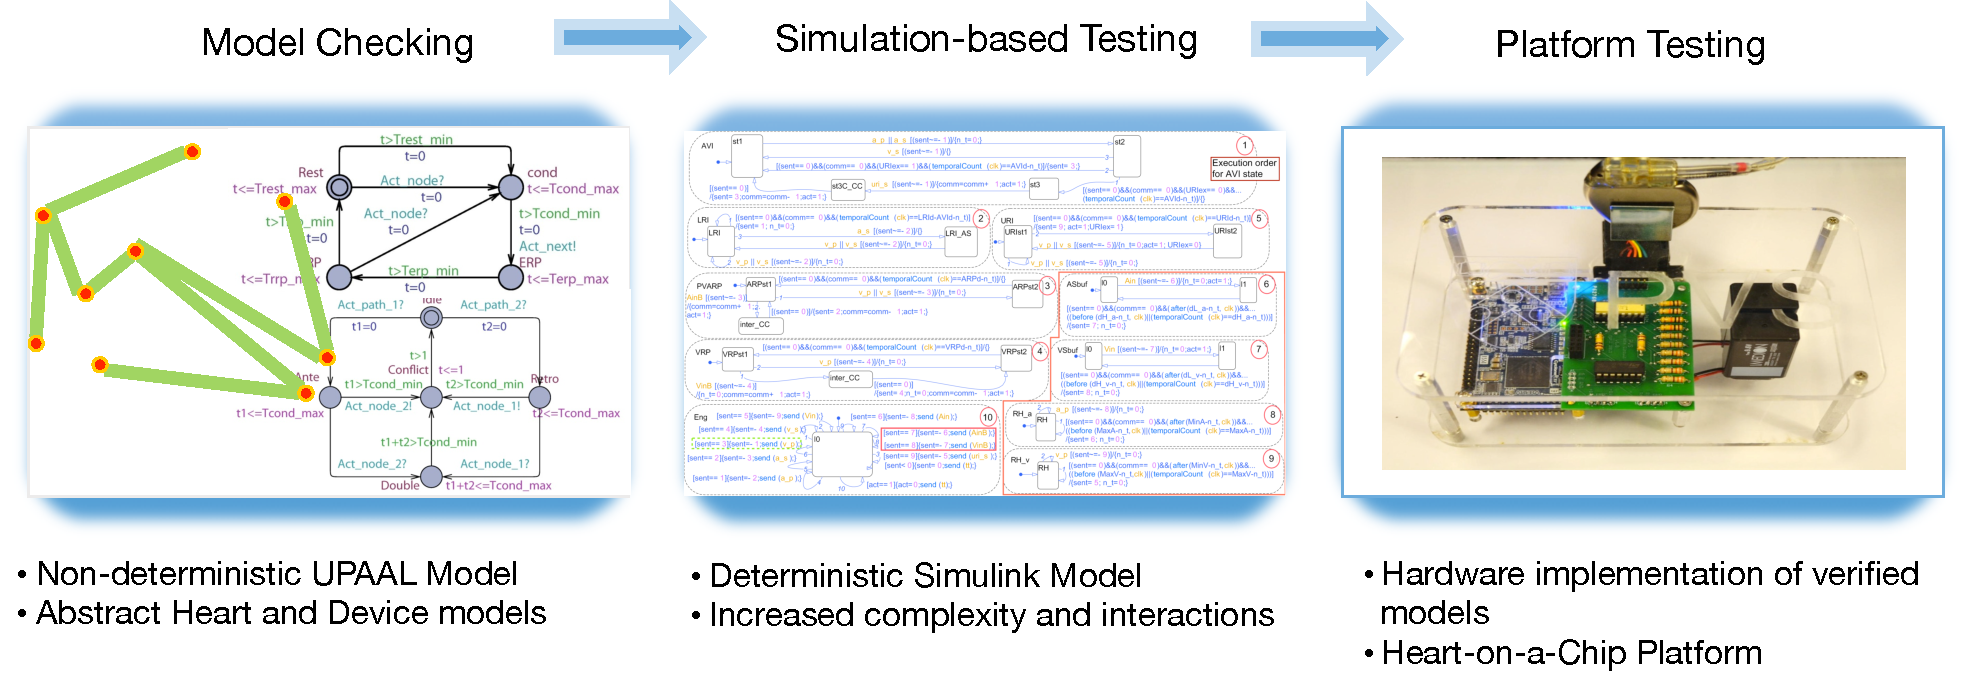
\includegraphics[width=\textwidth]{figs/fig4designtoimplementation.pdf}
	\caption{\small Model translation framework. The pacemaker design is verified using model checking and automatically translated into code implementation. Heart models are available at all levels}
	\label{fig:modelbaseddesign}
\end{figure}